\documentclass[10pt]{beamer}

\usepackage{polyglossia}
\usepackage{csquotes}
\usepackage{datetime}
\usepackage{fontspec}
\usepackage{microtype}
\usepackage{color}
\usepackage{url}
\usepackage{hyperref}
\usepackage{amsfonts}
\usepackage{amsmath}
\usepackage{amsthm}
\usepackage{subcaption}
\usepackage[backend=biber,style=iso-authoryear,sortlocale=en_US,autolang=other,bibencoding=UTF8]{biblatex}
\usepackage{booktabs}
\usepackage{graphics}
\usepackage{pifont}
\usepackage{ulem}
\usepackage{tikz}

\addbibresource{zotero.bib}

\setdefaultlanguage{english}
\setmainfont{TeX Gyre Termes}
\usetheme{Boadilla}
\usecolortheme{crane}
\setbeamertemplate{title page}[default][rounded=true,shadow=false]
\setbeamertemplate{section in toc}[ball unnumbered]
\setbeamertemplate{bibliography item}{}

\hypersetup{
	pdfencoding=auto,
	unicode=true,
	citecolor=green,
	filecolor=blue,
	linkcolor=red,
	urlcolor=blue
}

\makeatletter
\newcommand*{\currentSection}{\@currentlabelname}
\makeatother

%\newcommand{\mathmat}{\ensuremath{\mathbf}}

\title[Adaptive graph coarsening]
{
	Balancing performance and complexity with adaptive graph coarsening
}

\newdate{presentation}{22}{09}{2023}
\date[September 2023]{MLG @ ECML PKDD 2023, \displaydate{presentation}}

\author[Marek Dědič]
{
	\underline{Marek~Dědič}\inst{1}\inst{2},
	Lukáš~Bajer\inst{2},
	Pavel~Procházka\inst{2},
	Martin~Holeňa\inst{3}
}

\institute[CTU \& Cisco]
{
	\inst{1} Faculty of Nuclear Sciences and Physical Engineering, Czech Technical University in Prague \and
	\inst{2} Cisco Systems, Inc. \and
	\inst{3} Institute of Computer Science, Czech Academy of Sciences
}

% Title card
\AtBeginSection[]{
	\begin{frame}
		\vfill
		\centering
		\begin{beamercolorbox}[sep = 8pt,center,shadow = true,rounded = true]{title}
			\usebeamerfont{title}\insertsectionhead\par%
		\end{beamercolorbox}
		\vfill
	\end{frame}
}

%\AtBeginSection[]{
	%\begin{frame}{\currentSection}
		%\tableofcontents[currentsection]
	%\end{frame}
%}

\begin{document}

\begin{frame}
	\titlepage
\end{frame}

\begin{frame}{Motivation}
	\begin{figure}
		\centering
		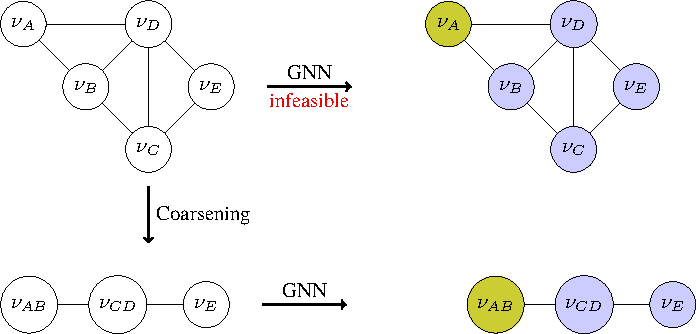
\includegraphics[width=0.8\linewidth]{images/coarsening-illustration/coarsening-illustration.pdf}
	\end{figure}
\end{frame}

\begin{frame}{The performance-complexity trade-off}
	\begin{figure}
		\centering
		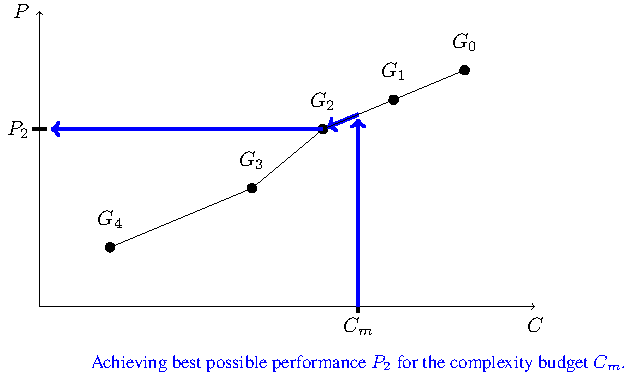
\includegraphics[width=0.8\linewidth]{images/performance-complexity/performance-complexity.pdf}
	\end{figure}
\end{frame}

\begin{frame}{Results}
	\begin{figure}
		\centering
		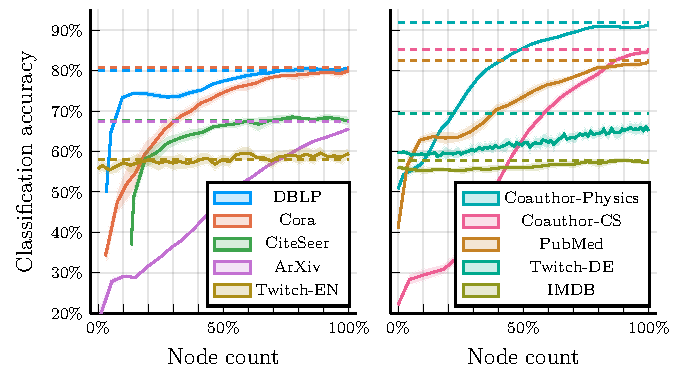
\includegraphics[width=0.8\linewidth]{images/adaptive-coarsening/adaptive-coarsening.pdf}
	\end{figure}
\end{frame}

\begin{frame}
	\titlepage
\end{frame}

\end{document}
